\documentclass[12pt]{article}

	\usepackage{lmodern}
\usepackage{amssymb}
\usepackage{graphicx}
\usepackage{amsmath}
\usepackage{multirow}
\usepackage{mathtools}
\usepackage{placeins}
\usepackage{lscape}
\usepackage{geometry}
\usepackage{dcolumn}
\usepackage[utf8]{inputenc}
\usepackage{hyperref}
\usepackage{tabularx}
\usepackage{nicematrix}
\usepackage{calc}
\usepackage{qtree}
\usepackage{tikz}
\usepackage{setspace}
\usepackage[utf8]{inputenc}

	
	\usepackage{fullpage} %sets 1-in margins
	\newcommand{\tab}{\hspace*{2em}} %creates a \tab command, gives you horizontal space

	\setlength\parindent{0em} %sets indent
	 %\pagestyle{empty} %turns off page numbering on all pages

\makeatletter
\setlength{\@fptop}{0pt}
\setlength{\@fpbot}{0pt plus 1fil}
\makeatother

\title{SOFR and Crowding-Out Effect}
\date{\today}
\author{Qian Wu}

\begin{document}

\maketitle

\section{Empirical Findings}
\subsection{Response of SOFR and LIBOR to Gov't Borrowing}
\begin{center}
\footnotesize
\begin{tabular}{@{\extracolsep{5pt}}lD{.}{.}{-3} D{.}{.}{-3} D{.}{.}{-3} D{.}{.}{-3} } 
\\[-1.8ex]\hline 
\hline \\[-1.8ex] 
\multicolumn{5}{c}{\textit{Panel A: Gov't debt outstanding as the measure of borrowing}} \\ 
\cline{1-5} \\
 & \multicolumn{4}{c}{\textit{Dependent variable:}} \\ 
 \cline{2-5} \\
\\[-1.8ex] & \multicolumn{2}{c}{SOFR} & \multicolumn{2}{c}{LIBOR} \\ 
\\[-1.8ex] & \multicolumn{1}{c}{(1)} & \multicolumn{1}{c}{(2)} & \multicolumn{1}{c}{(3)} & \multicolumn{1}{c}{(4)}\\ 
\hline \\[-1.8ex] 
$\Delta$log debt & 386.758^{***} & 381.218^{***} & -34.675^{**} & -33.695^{**} \\ 
  & (65.325) & (65.971) & (15.578) & (15.654) \\ 
SOFR(-1)  &  & 0.031 &  &  \\ 
  &  & (0.025) &  &  \\ 
LIBOR(-1)  &  &  &  & -0.144^{***} \\ 
  &  &  &  & (0.026) \\ 
  Constant & -0.241^{***} & -0.236^{***} & 0.011 & 0.011 \\ 
  & (0.076) & (0.077) & (0.018) & (0.018) \\ 
 \hline \\[-1.8ex] 
Observations & \multicolumn{1}{c}{1,526} & \multicolumn{1}{c}{1,520} & \multicolumn{1}{c}{1,489} & \multicolumn{1}{c}{1,464} \\ 
R$^{2}$ & \multicolumn{1}{c}{0.022} & \multicolumn{1}{c}{0.023} & \multicolumn{1}{c}{0.003} & \multicolumn{1}{c}{0.024} \\ 
Adjusted R$^{2}$ & \multicolumn{1}{c}{0.022} & \multicolumn{1}{c}{0.021} & \multicolumn{1}{c}{0.003} & \multicolumn{1}{c}{0.023} \\ 
Residual Std. Error & \multicolumn{1}{c}{2.929 (df = 1524)} & \multicolumn{1}{c}{2.933 (df = 1517)} & \multicolumn{1}{c}{0.689 (df = 1487)} & \multicolumn{1}{c}{0.686 (df = 1461)} \\ 
[.8ex]\hline 
\hline \\[-1.8ex] 
\multicolumn{5}{c}{\textit{Panel B: Treasuries outstanding as the measure of borrowing}} \\ 
\cline{1-5} \\
 & \multicolumn{4}{c}{\textit{Dependent variable:}} \\ 
 \cline{2-5} \\
\\[-1.8ex] & \multicolumn{2}{c}{SOFR} & \multicolumn{2}{c}{LIBOR} \\ 
\\[-1.8ex] & \multicolumn{1}{c}{(1)} & \multicolumn{1}{c}{(2)} & \multicolumn{1}{c}{(3)} & \multicolumn{1}{c}{(4)}\\ 
\hline \\[-1.8ex] 
$\Delta$log treasuries & 995.000^{***} & 994.614^{***} & -72.438^{***} & -66.848^{***} \\ 
  & (90.566) & (88.833) & (19.771) & (19.647) \\ 
SOFR(-1) &  & 0.177^{***} &  &  \\ 
  &  & (0.028) &  &  \\ 
LIBOR(-1) &  &  &  & -0.154^{***} \\ 
  &  &  &  & (0.030) \\ 
  Constant & -0.358^{***} & -0.314^{***} & 0.014 & 0.013 \\ 
  & (0.085) & (0.084) & (0.019) & (0.019) \\ 
 \hline \\[-1.8ex] 
Observations & \multicolumn{1}{c}{1,134} & \multicolumn{1}{c}{1,129} & \multicolumn{1}{c}{1,100} & \multicolumn{1}{c}{1,079} \\ 
R$^{2}$ & \multicolumn{1}{c}{0.096} & \multicolumn{1}{c}{0.129} & \multicolumn{1}{c}{0.012} & \multicolumn{1}{c}{0.036} \\ 
Adjusted R$^{2}$ & \multicolumn{1}{c}{0.096} & \multicolumn{1}{c}{0.127} & \multicolumn{1}{c}{0.011} & \multicolumn{1}{c}{0.034} \\ 
Residual Std. Error & \multicolumn{1}{c}{2.826 (df = 1132)} & \multicolumn{1}{c}{2.770 (df = 1126)} & \multicolumn{1}{c}{0.613 (df = 1098)} & \multicolumn{1}{c}{0.608 (df = 1076)} \\ 
\hline 
\hline \\[-1.8ex] 
\textit{Note:}  & \multicolumn{4}{r}{$^{*}$p$<$0.1; $^{**}$p$<$0.05; $^{***}$p$<$0.01} \\ 
\end{tabular} 
\end{center}


\newpage
\subsection{The Scarcity Value of Treasury Collateral}
\subsubsection{Segments of Markets Underlying SOFR}
The transactions underlying SOFR comprises two segments: bilateral repo and tri-party repo. In a bilateral repo, the settlement is handled directly by the trading parties rather than by a third-party clearing bank as in a triparty repo. Tri-party transactions are secured by General Collateral (GC) pools of accepted Treasury securities, any of which can be delivered as collateral by the cash borrower.  Unlike tri-pary transaction,  bilateral transactions feature Specific Collateral (SC) as lenders and borrowers can designate specific securities as collateral.  Therefore,  the incentive for lenders entering the bilateral repo market can be to seek a specific security.  A so-called collateral scarcity premium arises in bilateral transactions. \footnote{Infante and Saravay (2020) and D’Amico et al.  (2018) provide empirical evidence for treasury collateral scarcity.} \\
\begin{center}
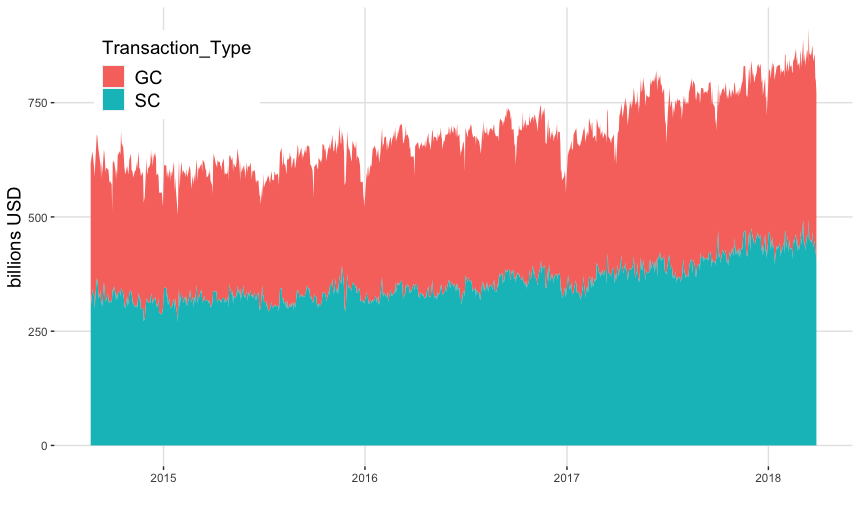
\includegraphics[scale=.5]{fig1.png}
\end{center}


\subsubsection{Treasuries Outstanding and Scarcity Value}
Intuitively,  when the volume of outstanding Treasuries is larger,  the Treasuries as collateral become less scarcity,  so the rate spread between bilateral repo transactions and tri-party repo transactions increases.  

\begin{center}
\begin{tabular}{@{\extracolsep{5pt}}lD{.}{.}{-3} D{.}{.}{-3} } 
\\[-1.8ex]\hline 
\hline \\[-1.8ex] 
 & \multicolumn{2}{c}{\textit{Dependent variable:}} \\ 
\cline{2-3} 
\\[-1.8ex] & \multicolumn{2}{c}{SC repo rate - GC repo rate} \\ 
\\[-1.8ex] & \multicolumn{1}{c}{(1)} & \multicolumn{1}{c}{(2)}\\ 
\hline \\[-1.8ex] 
$\Delta$log treasuries & 1,280.301^{***} & 1,321.397^{***} \\ 
  & (232.948) & (221.020) \\ 
$\Delta$log GC volume &  & -46.675^{***} \\ 
  &  & (4.473) \\ 
$\Delta$log SC volume&  & 6.483 \\ 
  &  & (4.377) \\ 
  Constant & -0.236 & -0.238 \\ 
  & (0.225) & (0.212) \\ 
 \hline \\[-1.8ex] 
Observations & \multicolumn{1}{c}{899} & \multicolumn{1}{c}{899} \\ 
R$^{2}$ & \multicolumn{1}{c}{0.033} & \multicolumn{1}{c}{0.138} \\ 
Adjusted R$^{2}$ & \multicolumn{1}{c}{0.031} & \multicolumn{1}{c}{0.135} \\ 
Residual Std. Error & \multicolumn{1}{c}{6.591 (df = 897)} & \multicolumn{1}{c}{6.230 (df = 895)} \\ 
\hline 
\hline \\[-1.8ex] 
\textit{Note:}  & \multicolumn{2}{r}{$^{*}$p$<$0.1; $^{**}$p$<$0.05; $^{***}$p$<$0.01} \\ 
\end{tabular} 
\end{center}


\newpage
\subsection{Local Projection}
To show that the extra response in SOFR with respect to government borrowing is significantly large and persistent,
I conduct time series analysis using Local Projection with monthly data covering the period
between 2014/08 and 2019/12. In the first stage, I identify the government borrowing shock
using the following strategy:
\begin{align*}
  b_t=\alpha_0+\alpha_1t+\alpha_2t^2+A(L)X_{t-1}+\epsilon_t^b,
\end{align*}
where $b_t$ denotes log(govt debt); $X_t$ denotes controls including six lags of log(govt debt), log(industrial production), and log(stock price)
\footnote{Identifying the government borrowing shock using twelve lags obtains similar result.}; and
$\hat{\epsilon}_t^b$ is adopted as the identified borrowing shock. In the second stage, I estimate the following equation to generate the impulse response functions of SOFR and LIBOR to a standard deviation of government
borrowing shock.
\begin{align*}
  r_{t+h}=\beta_0+\psi_h \hat{\epsilon}_t^b +\Gamma(L)Z_{t-1}+u_{t+h},
\end{align*}
where $r_{t+h}$ denotes SOFR or LIBOR spread at horizon h; $Z_{t-1}$ denotes controls including three lags of SOFR or LIBOR spread, log(govt debt), and log(industrial production).
The IRFs are given in graphs below. Note that SOFR spread exhibits a positive and persistent response to government
borrowing shock for as long as 12 horizons (months) after the shock happens. A simple numerical analysis reveals that a 1-percentage increase in government debt outstanding, which is equivalent to a
0.75-percentage change in GDP \footnote{In dollar value, this is roughly 146 billion.}, results in a 0.8-bps rise in SOFR right after the borrowing shock. 
This effect remains positive within the following 12 months and peaks at 3.3-bps in 8 months after the shock.
On the other hand, LIBOR spread responds ambiguously. Two robustness checks are conducted. In the first alternative specification, I replace industrial production with unemployment rate as a measure of output,
the resulting IRFs are very similar. Also, in order to exclude the possible effect from price level, CPI is employed as a control in the second alternative specification, and the results remain unchanged.
\begin{center}
  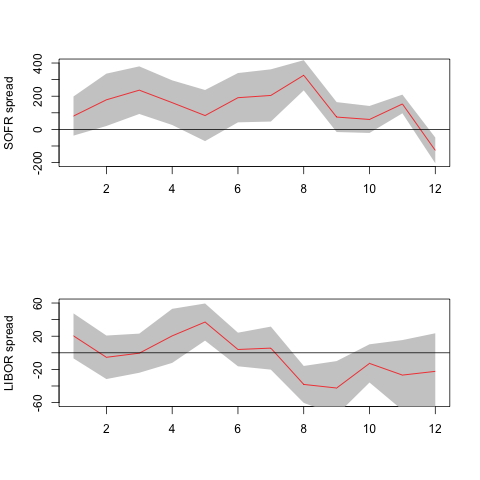
\includegraphics[scale=0.8]{../lp/results/irfs.png}
\end{center}

\newpage
\section{Model}
The theoretical model is built based on Walque, Pierrard, and Rouabah (2010). Departing from a perfectly competitive credit market between households and firms, in this paper the direct borrowing between firms and households is not feasible and the capital must flow through an interbank lending market.
Firms borrow uninsuredly from the merchant banks for business capital, and commercial banks are financed using insured interbank loans lent by deposit banks. For commercial banks to borrow on the interbank market, they must use government bonds as collateral. This creates an additional motivation
for commercial banks to hold government bonds, besides the profit motivation. Firms and merchant banks are allowed to default, creating risk premiums on top of the risk free rate. 


\subsection{Household's Problem}
Households choose consumption $C_t$ and deposits $D_t$ to maximize their expected lifetime utility subject to flow budget constraint. I assume exogenous labor supply $N$ to simplify the analysis.
Each period households receive wage payment $w_tN$, deposit payment $D_{t-1}$, and dividend payments $d^t_D$ from deposit banks, $d_t^C$ from commercial banks, and $d_t^F$ from firms.
Finally, households have to pay a lump-sum tax $T_t$.
\begin{align}
  &\max_{\{c_t, D_t\}} E \sum_{t=0}^{\infty} \beta^t logC_t ,\\
  s.t. \nonumber \\
  &C_t+\frac{D_t}{1+r_t}+T_t=w_tN+D_{t-1}+d_t^D+d_t^C+d_t^F
\end{align}
The FOC is 
\begin{align}
  \frac{1}{C_t}&=\beta (1+r_t)E_t\big(  \frac{1}{C_{t+1}}\big)
\end{align}


\subsection{Deposit Bank's Problem}
Deposit banks demand deposit from households, and they do collateralized lendings to commercial banks through the interbank lending market.
Each period, deposit banks choose deposit demand $D_t$ and interbank lending supply $I_t$ to maximize profits.  Interbank lending requires
collateral in the form of government bonds. For the part of lendings on which the merchant banks choose to default, the deposit banks will recover
a fraction $\theta$ of the collateralized assets. Notice that I assume a quadratic payment adjustment cost to avoid corner solutions.
\begin{align}
  &\max_{\{D_t, I_t, d_t^D\}} E \sum_{t=0}^{\infty} \{M_t[d_t^D-(\frac{d_t^D-\bar{d}^D}{2})^2]\} ,\\
  s.t. \nonumber \\
  &d_t^D=\gamma_t^I I_{t-1}+\frac{D_t}{1+r_t}-D_{t-1}-\frac{I_t}{1+r_t^I}+ \theta(1-\gamma_{t-1}^I)I_{t-2},\\
  &I_t=D_t
\end{align}
The FOC is 
\begin{align}
  \frac{M_t}{1+r_t^I}(1-\frac{d_t^D-\bar{d}^D}{2})&=E_t  \big[M_{t+1}\gamma_{t+1}^I (1-\frac{d_{t+1}^D-\bar{d}^D}{2})\big]
\end{align}


\subsection{Commercial Bank's Problem}
Commercial banks demand insured borrowing from deposit banks with government bonds as the collateral. In the meantime, they issue uninsured business loans to firms to earn interests.
Each period commercial banks choose interbank lending demands $I_t$, government bonds holding $B_t$, business loan supply $L_t$, and repayment rate $\gamma_t^I$ to maximize its profits. 
I continue to assume a quadratic payment adjustment cost for commercial banks. To borrow on the interbank market, commercial banks must obey the collateral requirement, they cannot borrow
more than the bonds they hold. What's more, to simplify the problem, I assume that commercial banks borrow at their limits. 
Since the government bond is a risk-free asset, in this paper I do not apply a haircut on the collateral.
In case of default, the commercial banks will lose a fraction $\theta$ of their collateral. Other pecuniary costs such as higher searching costs to obtain future loans is given by a quadratic function of the defaulted borrowing.
\begin{align}
  &\max_{\{I_t, B_t, L_t, \gamma_t^I, d_t^C\}} E \sum_{t=0}^{\infty} \{M_t[d_t^C-(\frac{d_t^C-\bar{d}^C}{2})^2]\} ,\\
  s.t. \nonumber \\
  &d_t^C=\gamma_t^L L_{t-1}+\frac{I_t}{1+r_t^I}-\gamma_t^I I_{t-1}-\frac{L_t}{1+r_t^L} \nonumber \\
  & \hspace{3cm}-\theta(1-\gamma_{t-1}^I)I_{t-2}-\xi_C(1-\gamma_t^I)+B_{t-1}-\frac{B_t}{1+r_t^B}, \\
  &I_t= B_t 
\end{align}
The FOCs are 
\begin{align}
  &M_t (1-\frac{d_t^C-\bar{d}^C}{2})(\frac{1}{1+r_t^I}-\frac{1}{1+r_t^B}) \nonumber \\
  & \hspace{5mm} = E_t \bigg\{ M_{t+1} (1-\frac{d_{t+1}^C-\bar{d}^C}{2})(\gamma_{t+1}^I-1)+ M_{t+2} (1-\frac{d_{t+2}^C-\bar{d}^C}{2}) [\theta(1-\gamma_{t+1}^I)] \bigg\}, \\
  &\frac{M_t}{1+r_t^L}(1-\frac{d_t^C-\bar{d}^C}{2})=E_t \big[M_{t+1} \gamma_{t+1}^L (1-\frac{d_{t+1}^C-\bar{d}^C}{2})\big], \\
  &M_t (1-\frac{d_t^C-\bar{d}^C}{2})(B_{t-1}-\xi_C)=E_t \bigg\{ M_{t+1} (1 -\frac{d_{t+1}^C-\bar{d}^C}{2})(\theta B_{t-1}) \bigg\}
\end{align}


\subsection{Firm's Problem}
Firms require uninsured business loans from commercial banks to finance the production. They can default on business loans with a penalty. Each period firms choose 
labor demand $N_t$, business loan demand $L_t$, and repayment rate $\gamma_t^L$ to maximize profits. 
\begin{align}
  &\max_{\{N_t, L_t, \gamma_t^L, d_t^F, K_t\}} E \sum_{t=0}^{\infty} \{ M_t[d_t^F-(\frac{d_t^F-\bar{d}^F}{2})^2]\} ,\\
  s.t. \nonumber \\
  &K_t=(1-\delta)K_{t-1}+\frac{L_t}{1+r_t^L}, \\
  &d_t^F=F(K_t, N_t)-w_tN_t-\gamma_t^L L_{t-1}-\xi_F(1-\gamma_t^L)
\end{align}
The FOCs are 
\begin{align}
  &F_N(K_t, N_t)=w_t, \\
  &M_t (1-\frac{d_t^F-\bar{d}^F}{2})F_K(K_t, N_t) \nonumber \\
  &\hspace{5mm} = E_t \bigg\{ M_{t+1} (1-\frac{d_{t+1}^F-\bar{d}^F}{2} )(1+r_t^L)\gamma_{t+1}^L
  -(1-\delta)M_{t+2} (1 -\frac{d_{t+2}^F-\bar{d}^F}{2})(1+r_{t+1}^L)\gamma_{t+2}^L \bigg\}, \\
  &\xi_F = L_{t-1}
\end{align}


\subsection{Government Budget Constraint}
Government runs a balanced budget. Each period it pays back the government bonds issued at last period and consume goods. 
To finance spending, the government will issue new bonds and levy lump sum tax on households.
\begin{align}
  G_t+B_{t-1}=\frac{B_t}{1+r_t^B}+T_t
\end{align}


\subsection{General Equilibrium}
To simplify the analysis, I assume that lump-sum tax $T_t$ is fixed at $T$. The government spending is given exogenously as
\begin{align}
  G_t=\rho G_{t-1}+\sigma_t.
\end{align}
The general equilibrium is characterized as follows:\\
Allocation paths $\{C_t, D_t, I_t, B_t, d_t^D, L_t, \gamma_t^I, d_t^C, \gamma_t^L, d_t^F, K_t\}$, price paths $\{ r_t, r_t^I, r_t^L, r_t^B, w_t\}$, and
government policies $\{G_t, B_t\}$ such that \\
(1) First order conditions and budget constraints satisfy;\\
(2) Labor market, deposit market, interbanking lending market, and business loan market all clear;\\
(3) Government budget constraint satisfies;


\section{Steady State}
The steady state version of this general equilibrium model is given by the following 16 equations.
\begin{align}
  &r=1/\beta-1, \\
  &B=\xi_C/(1-\beta \theta), \\
  &I=B,\\
  &\gamma^I=\frac{1-(T-G)(1-\beta \theta)/ \xi_C+\beta (\beta \theta-1)}{\beta^2 \theta},\\
  &r^I=1/(\beta \gamma^I)-1,\\
  &r^B=\frac{1}{\beta[1-\beta \theta(1-\gamma^I)]}-1,\\
  &D=I,\\
  &d^D=[(1-\theta-\beta)\gamma^I+\theta]I+(\beta-1)D,\\
  &L=\xi_F,\\
  &K=\bigg(\frac{1-(1-\delta) \beta} {\alpha}\bigg)^{1/(\alpha-1)}N,\\
  &\gamma^L=\delta K/(\beta L),\\
  &r^L=1/(\beta \gamma ^L)-1, \\
  &w=(1-\alpha)(K/N)^{\alpha},\\
  &d^C=\gamma^L L+(\beta-1)\gamma^I I-L\beta \gamma^L-\theta (1-\gamma^I)I-\xi_C(1-\gamma^I)+B-B/(1+r^B),\\
  &d^F=K^{\alpha}N^{1-\alpha}-wN-\gamma^L L-\xi_F(1-\gamma^L),\\
  &C=(1-\beta)D+wN+d^D+d^C+d^F-T.x
\end{align}





\end{document}

